\chapter{Resultados e Discussões}
\label{chapter:results}

% BASE
% termos e temas coletados
% tabela de escolha de emoticons
% volume da base taggeada automaticamente
% relacao usuarios (retweets)
% status dos grafos
% volume da base de teste

A etapa de coleta de dados captou aproximadamente 9,2 milhões de tweets únicos
entre 2018 e 2019.
Parte desses tweets foi coletada da amostragem do conjunto total de mensagens
publicadas e outra parte da amostrada dentre os tópicos: \textit{Libertadores,
ENEM, Amazônia} e \textit{Rock in Rio}.
Nessa base há aproximadamente 45 milhões de retweets, fornecendo a conexão entre
pessoas que será utilizada para montar a rede de usuários.

Para anotação automática foram identificados os emoticons mais frequentes da
base de dados e classificados manualmente entre positivos e negativos,
desconsiderando os neutros.
A Tabela~\ref{tab:emoticons} mostra as classes dos emoticons selecionados.
Com esse conjunto de emoticons 580 mil tweets foram anotados por supervisão
distante, dentre os quais 130 mil marcados como negativos e 450 mil marcados como
positivos.

\begin{table}[h]
    \begin{center}
        \begin{tabular}{| l | c |}
        \hline
        \textbf{Classe} & \textbf{Emoticons} \\ \hline
        Positiva &
            
\includegraphics[height=1em]{images/emojis/2764}
            
\includegraphics[height=1em]{images/emojis/1F602}
            %\includegraphics[height=1em]{images/emojis/1F5A4}
            %\includegraphics[height=1em]{images/emojis/1F923}
            
\includegraphics[height=1em]{images/emojis/1F60D}
            
\includegraphics[height=1em]{images/emojis/2665}
            %\includegraphics[height=1em]{images/emojis/1F970}
            
\includegraphics[height=1em]{images/emojis/1F605}
            
\includegraphics[height=1em]{images/emojis/1F601}
            %\includegraphics[height=1em]{images/emojis/1F92D}
            
\includegraphics[height=1em]{images/emojis/1F618}
            
\includegraphics[height=1em]{images/emojis/1F609}
            
\includegraphics[height=1em]{images/emojis/1F496}
            
\includegraphics[height=1em]{images/emojis/1F495}
            
\includegraphics[height=1em]{images/emojis/1F606}
            %\includegraphics[height=1em]{images/emojis/1F973}
            
\includegraphics[height=1em]{images/emojis/1F499}
            
\includegraphics[height=1em]{images/emojis/1F389}
            
\includegraphics[height=1em]{images/emojis/1F61D}
            
\includegraphics[height=1em]{images/emojis/1F49A}
            
\includegraphics[height=1em]{images/emojis/1F49C}
            %\includegraphics[height=1em]{images/emojis/2763}
            
\includegraphics[height=1em]{images/emojis/1F60A}
            
\includegraphics[height=1em]{images/emojis/1F60B}
            %\includegraphics[height=1em]{images/emojis/1F917}
        \\ \hline
        Negativa &
            
\includegraphics[height=1em]{images/emojis/1F62D}
            
\includegraphics[height=1em]{images/emojis/1F645}
            %\includegraphics[height=1em]{images/emojis/1F926}
            
\includegraphics[height=1em]{images/emojis/1F621}
            
\includegraphics[height=1em]{images/emojis/1F614}
            %\includegraphics[height=1em]{images/emojis/1F92C}
            %\includegraphics[height=1em]{images/emojis/1F92E}
            
\includegraphics[height=1em]{images/emojis/1F629}
            
\includegraphics[height=1em]{images/emojis/1F622}
            
\includegraphics[height=1em]{images/emojis/1F620}
            
\includegraphics[height=1em]{images/emojis/1F612}
            
\includegraphics[height=1em]{images/emojis/1F624}
            
\includegraphics[height=1em]{images/emojis/1F494}
            
\includegraphics[height=1em]{images/emojis/1F62A}
            
\includegraphics[height=1em]{images/emojis/1F625}
            
\includegraphics[height=1em]{images/emojis/1F62B}
            
\includegraphics[height=1em]{images/emojis/1F630}
        \\ \hline
        \end{tabular}
        \caption{Emoticons selecionados para aplicação de supervisão distante.}
        \label{tab:emoticons}
    \end{center}
\end{table}

A rede de usuários foi formada por retweets entre usuários.
Os 45 milhões de retweets formam uma rede de 28 milhões de arestas únicas
conectando 5,5 milhões de vértices, representando uma densidade de
$9,4\times10^{-7}$.
O coeficiente de clusterização global é de $9,6\times10^{-4}$, portanto,
havendo um vizinho em comum o nó tem 1000 vezes mais chance de estar conectado a
outro nó do que quando ambos não compartilham conexões.
Aproximadamente 4,5\% dos nós pertencem a componente fortemente conexa, ou seja,
subgrafo direcional em que existe um caminho entre todos os vértices.
Enquanto 97\% dos nós pertencem a componente fracamente conexa, que leva em
consideração o subgrafo não direcional.
Observa-se que a rede inteira é formada praticamente por uma única componente
enquanto os outros 3\% dos usuários estão distribuídos em um grande
volume de pequenas componentes.
A Figura~\ref{fig:graph_ccdf} mostra as distribuições de grau dos vértices.
Analisa-se que tanto a distribuição de grau de entrada quanto a de saída tem
caudas longas apesar da curva da distribuição de de grau de entrada ser
significativamente mais extensa.
Ressalta-se também que mais que 80\% dos nós tem grau de entrada 0, ou seja,
são usuários que não receberam nenhum retweets.
A Figura~\ref{fig:graph_distance} mostra a distribuição de distância entre os
nós da rede, que tem média $8,8$.
Conclui-se portanto que dentre os dados captados formou-se uma rede com número
significativo de usuários e possuí características comumente observadas em redes
como a formação de \textit{hubs}, pequena distância média e grande componente
conexa.

\begin{figure}[h]
\begin{center} {
    \begin{center}
    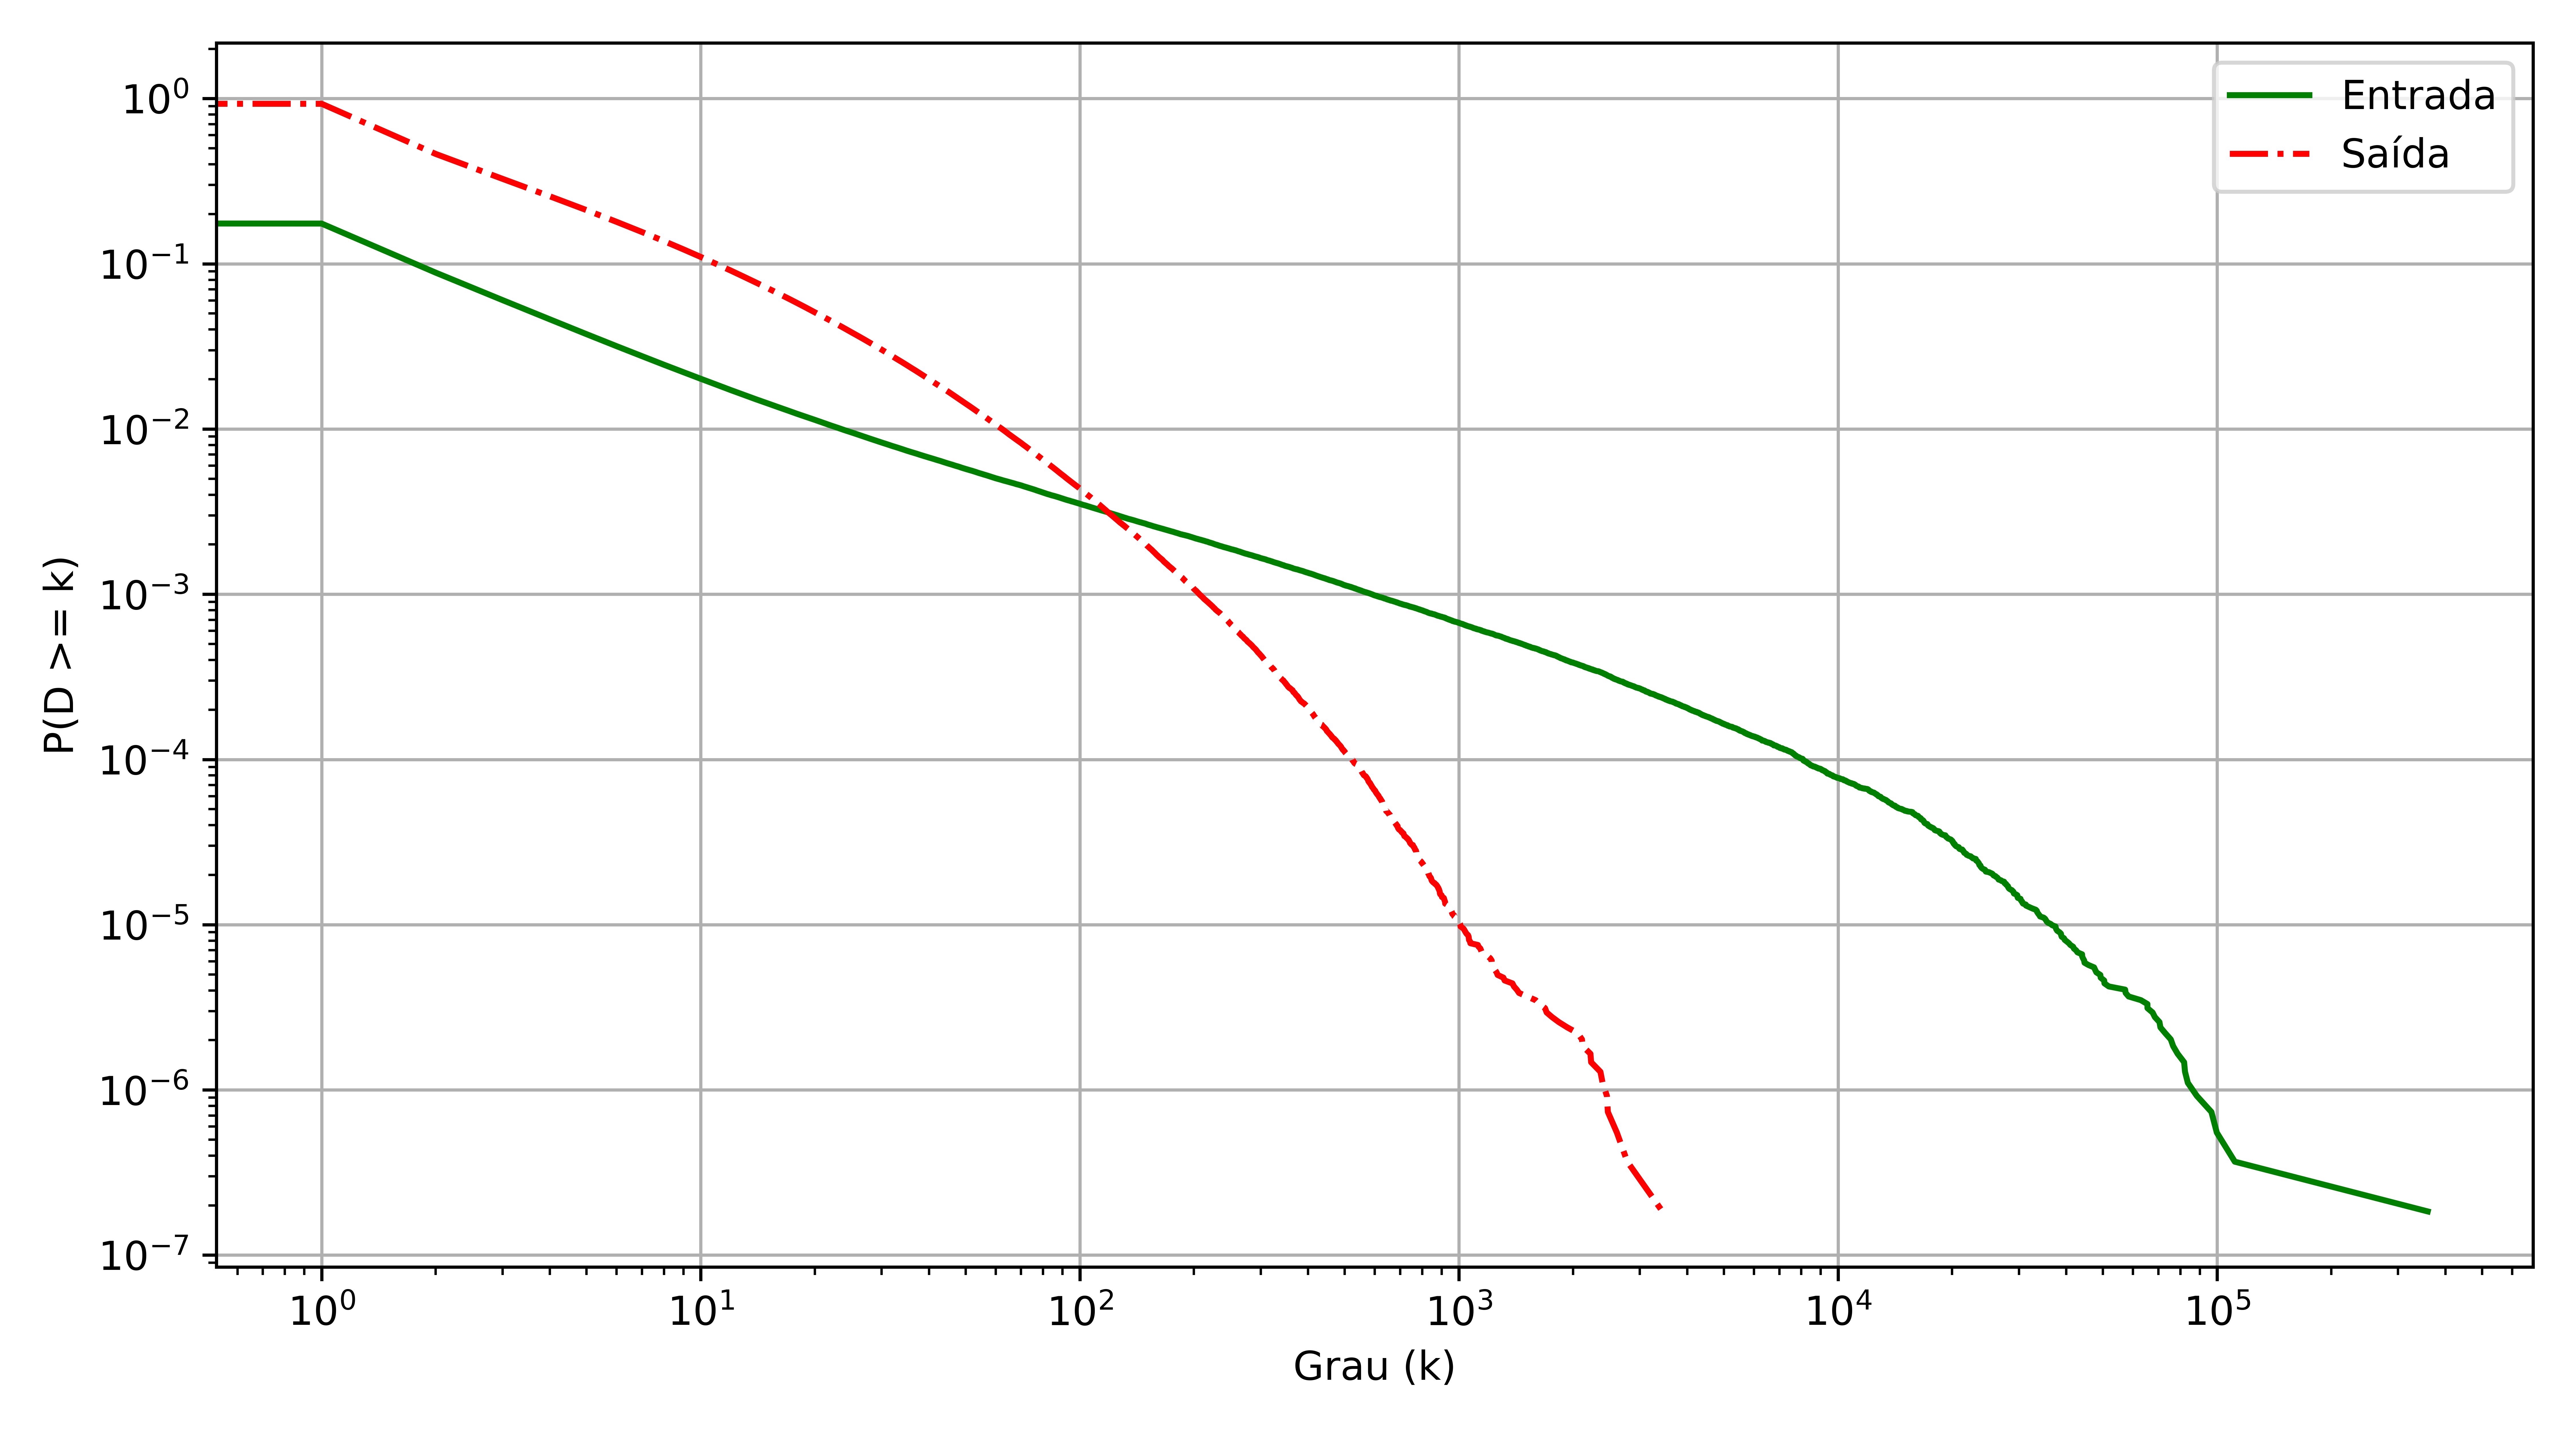
\includegraphics[scale=0.65]{images/graph_ccdf.png}
    \caption{Gráfico da \textit{CCDF (complementary cumulative distribution function)}
             dos graus de entrada e saída da rede de usuários.
             O eixo horizontal representa o grau $k$ enquanto o eixo vertical
             demonstra a probabilidade de um vértice ter grau pelo menos $k$.}
    \label{fig:graph_ccdf}
    \end{center}
}
\end{center}
\end{figure}

\begin{figure}[h]
\begin{center} {
    \begin{center}
    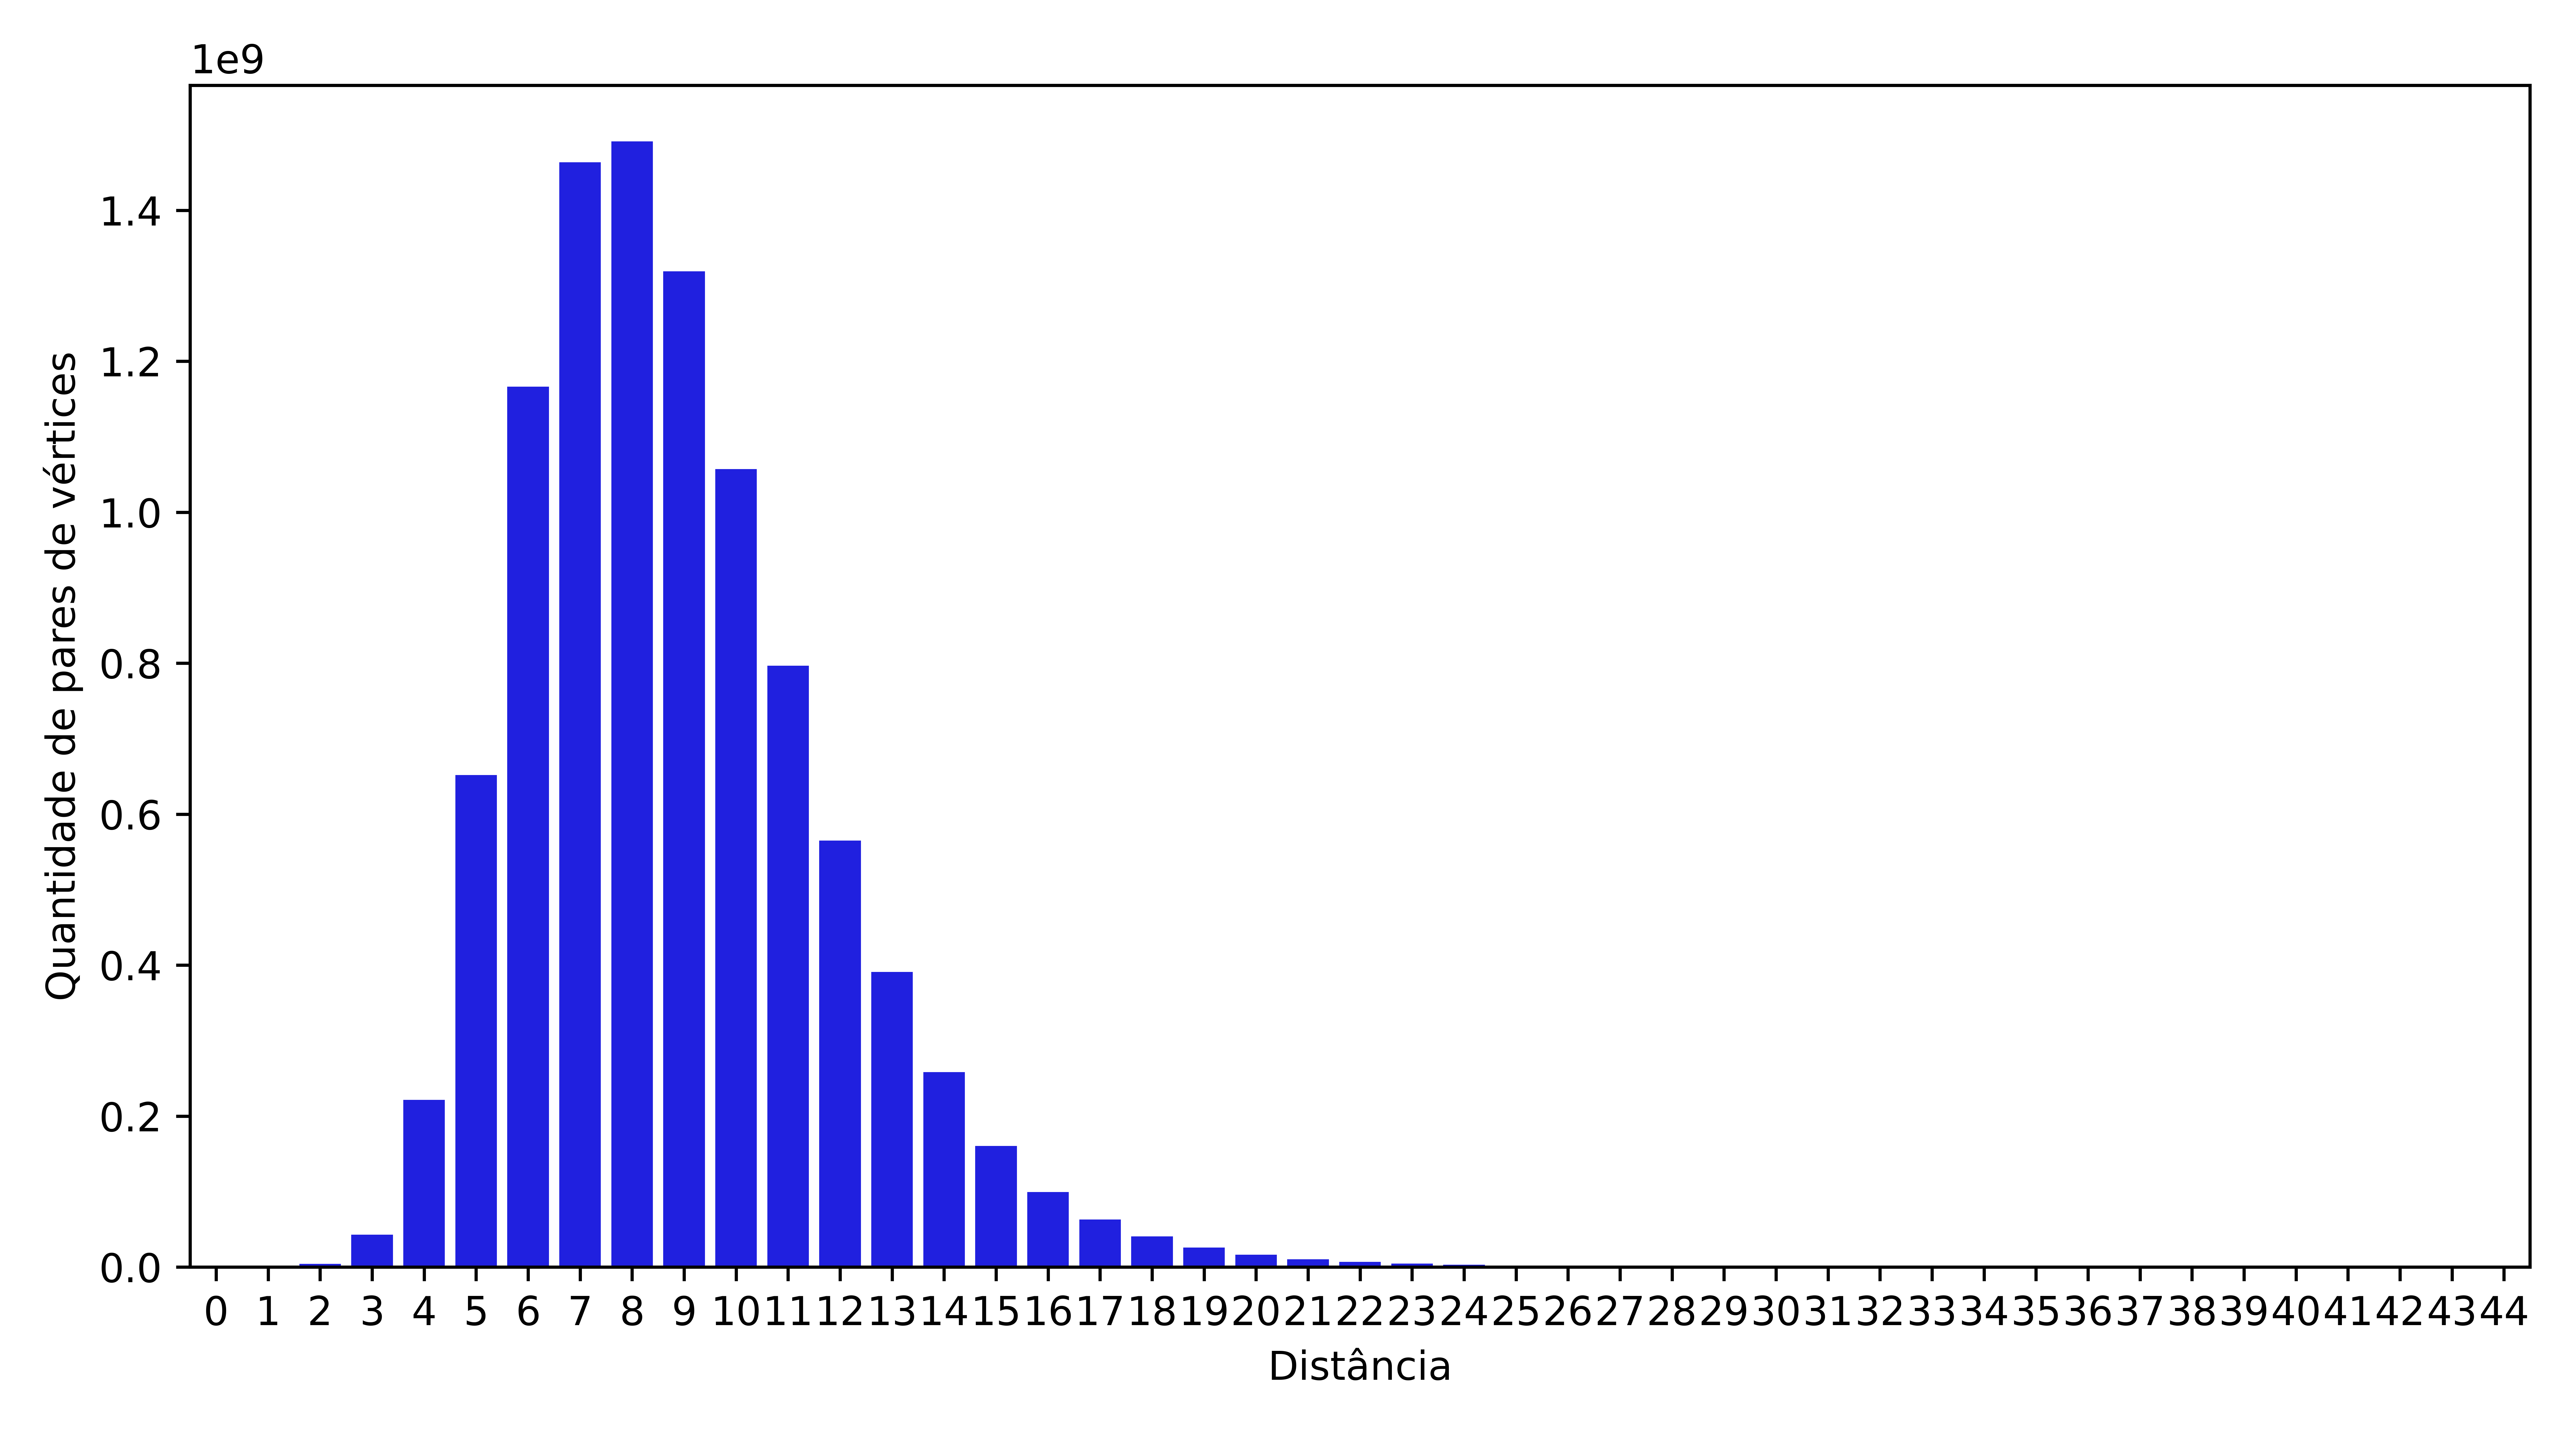
\includegraphics[scale=0.65]{images/graph_distance.png}
    \caption{Contagem de eventos da distância entre pares de nós da rede de usuários.}
    \label{fig:graph_distance}
    \end{center}
}
\end{center}
\end{figure}

Uma vez finalizada a etapa de coleta dos dados, o processo de anotação e a
formação da rede de usuários, se prosseguiu para a etapa do classificador de
sentimento textuais.
Esses classificadores serão usados como base de comparação para avaliar a
eficiência dos classificadores multimodais.

\section{Classificadores Textuais Lineares}

Os primeiros classificadores textuais treinados foram os por Naïve Bayes e SVM.
Nesse caso, ambos usaram a representação Bag-of-Words.
O vocabulário formado a partir da base coletada é composto por 127 mil termos.
O treinamento do algoritmo de Naïve Bayes multinomial foi feito utilizando
validação cruzada por K-partições, no total de 10 partições, sob os dados de
treinamento anotados com supervisão distante. O parâmetro de suavização foi
escolhido por \textit{grid search}, de maneira a maximizar a área sob a curva ROC.
A Figura~\ref{fig:nb_grid} mostra a resposta do modelo para os diferentes fatores
de suavização testados.

\begin{figure}[h!]
\begin{center} {
    \begin{center}
    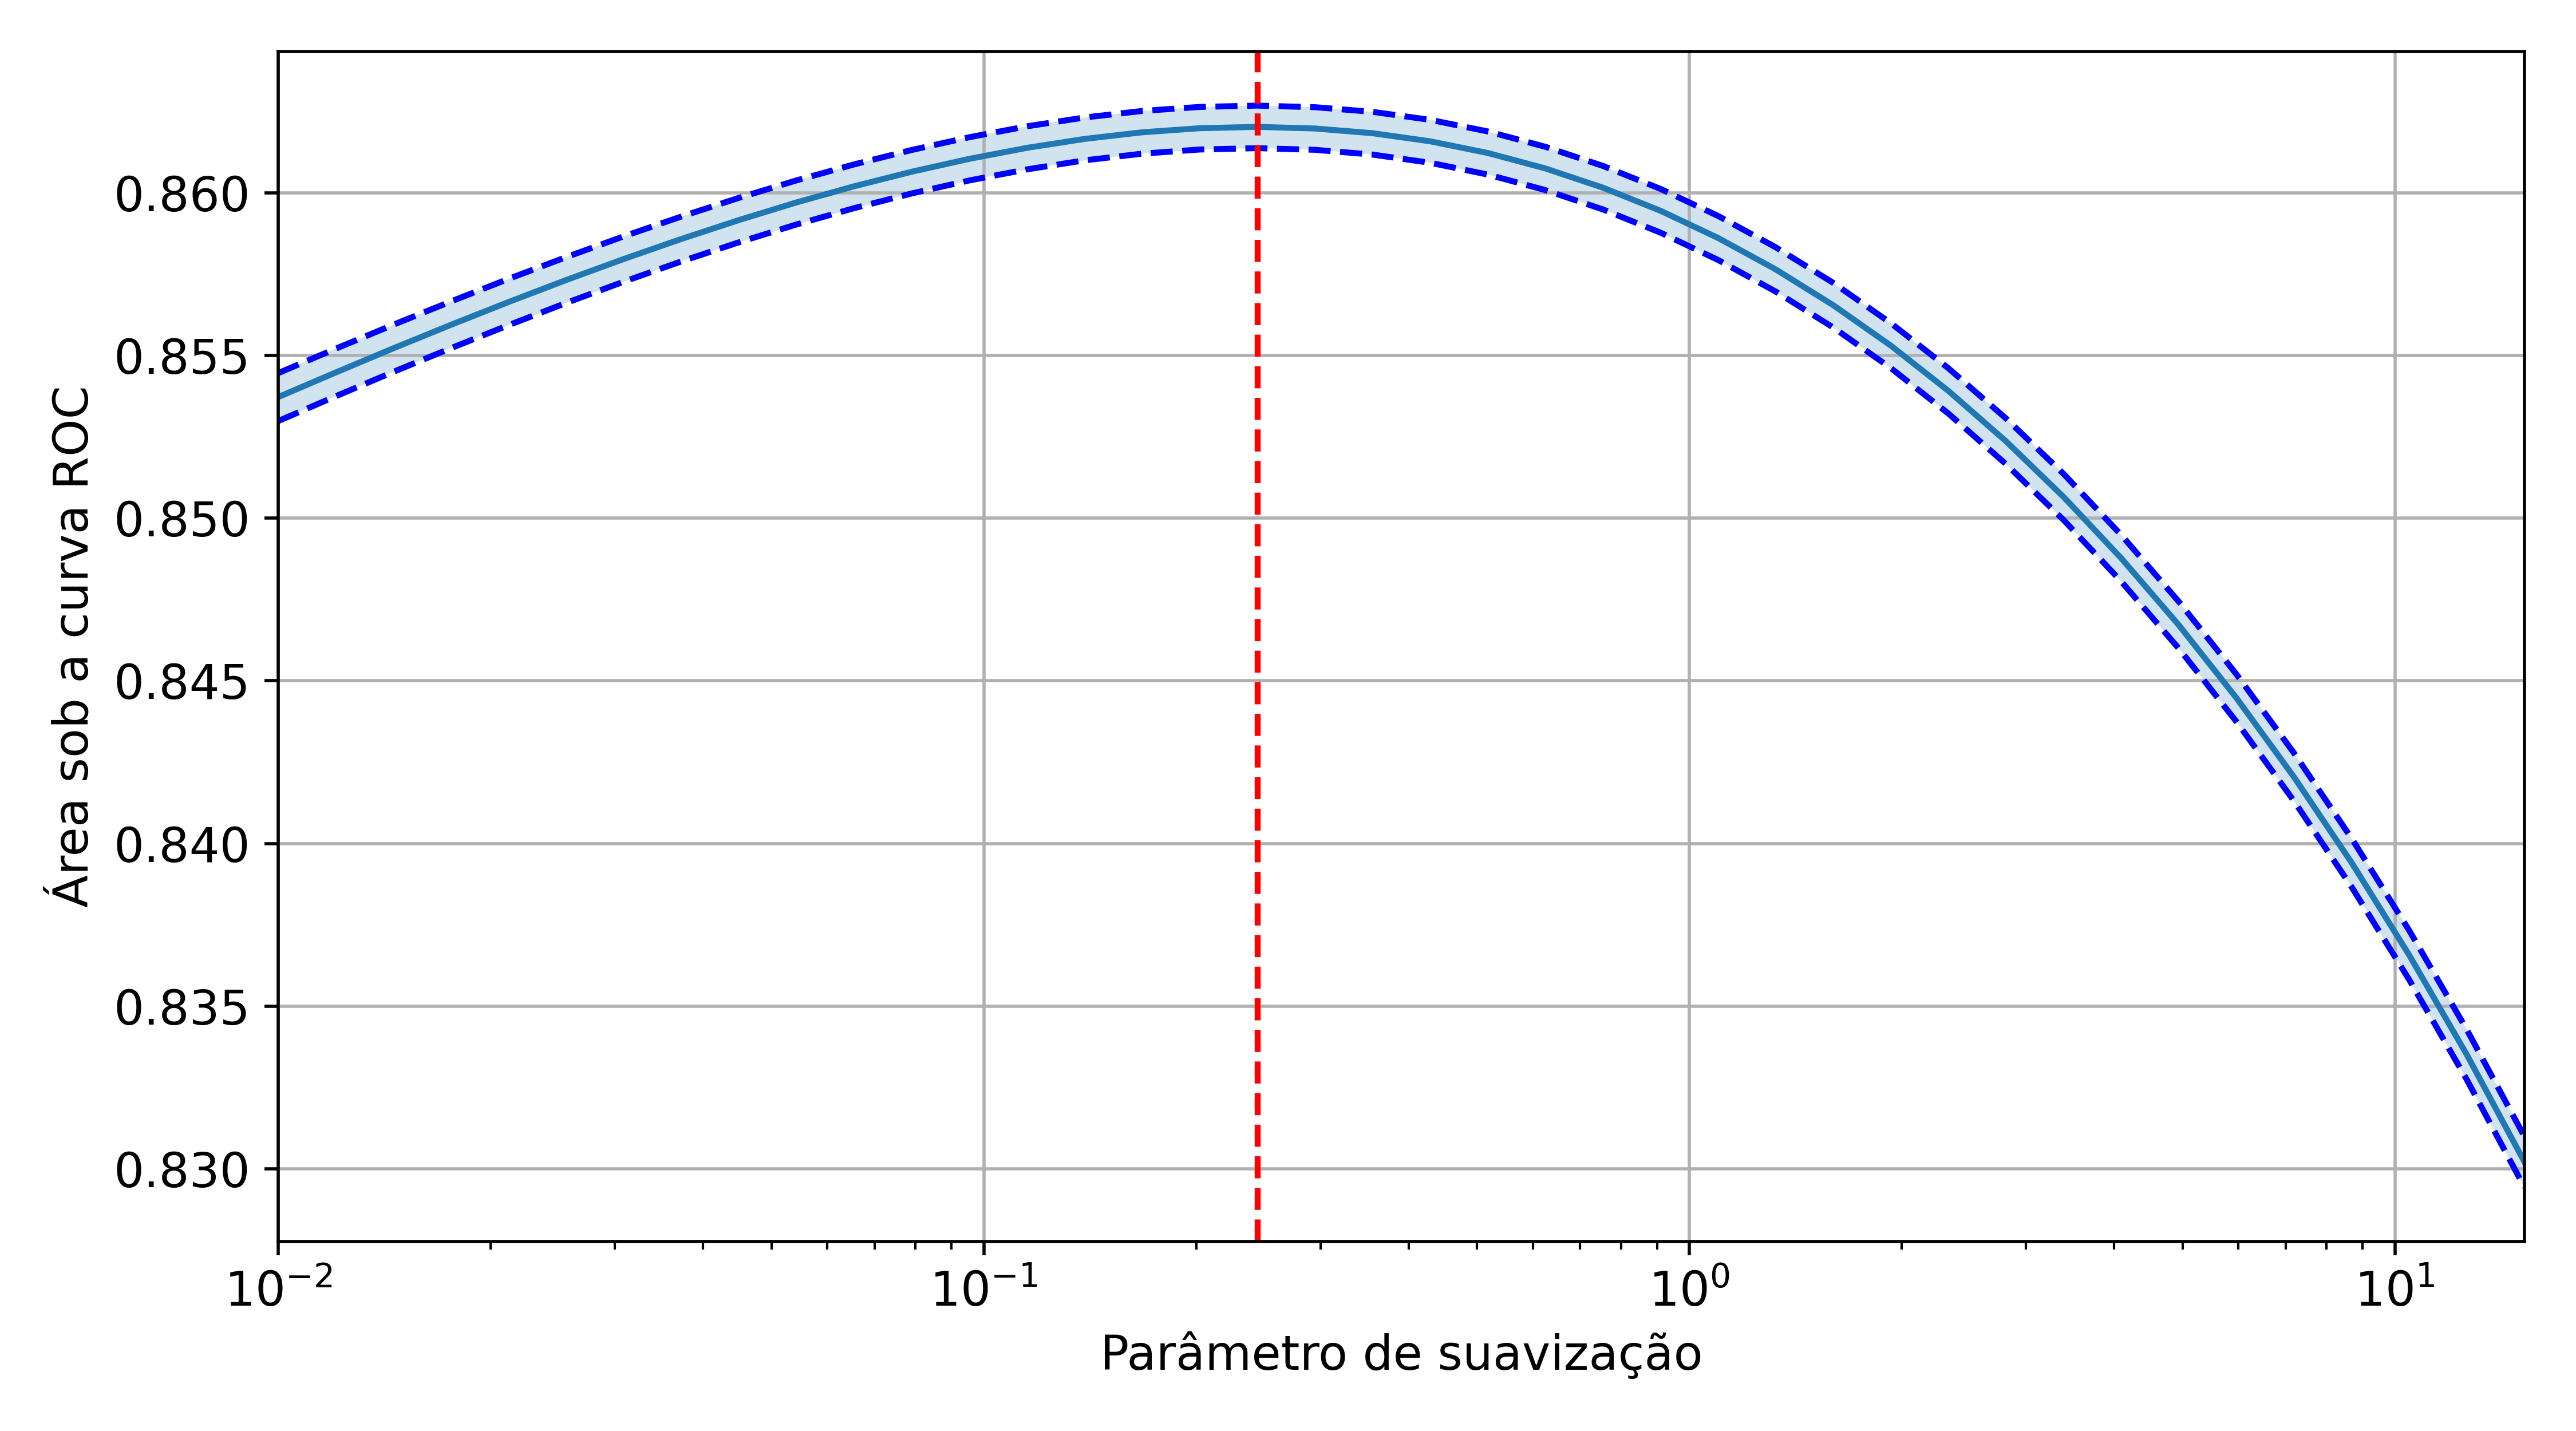
\includegraphics[scale=0.65]{images/nb_grid.png}
    \caption{Resposta do modelo de Naïve Bayes a variação do parâmetro de suavização.
             A linha cheia representa a média dos valores das 10 partições
             enquanto a área em azul, limitada pela linha hachurada, representa um desvio padrão.
             A linha vertical vermelha ressalta o parâmetro de maior média.}
    \label{fig:nb_grid}
    \end{center}
}
\end{center}
\end{figure}

O hiperparâmetro selecionado foi o de valor $0,244$, que obteve AUC de $0,862 \pm 0,002$.
Uma vez selecionado o melhor modelo na base de treino, o mesmo foi avaliado com
os dados da base de teste, que foram anotados manualmente.
A Figura~\ref{fig:nb_roc} apresenta a curva ROC dos dados de treino.
Observa-se que o mesmo modelo ao ser aplicado aos dados de teste tem resultado
de $0,801$ de área sob curva ROC.

\begin{figure}[h!]
\begin{center} {
    \begin{center}
    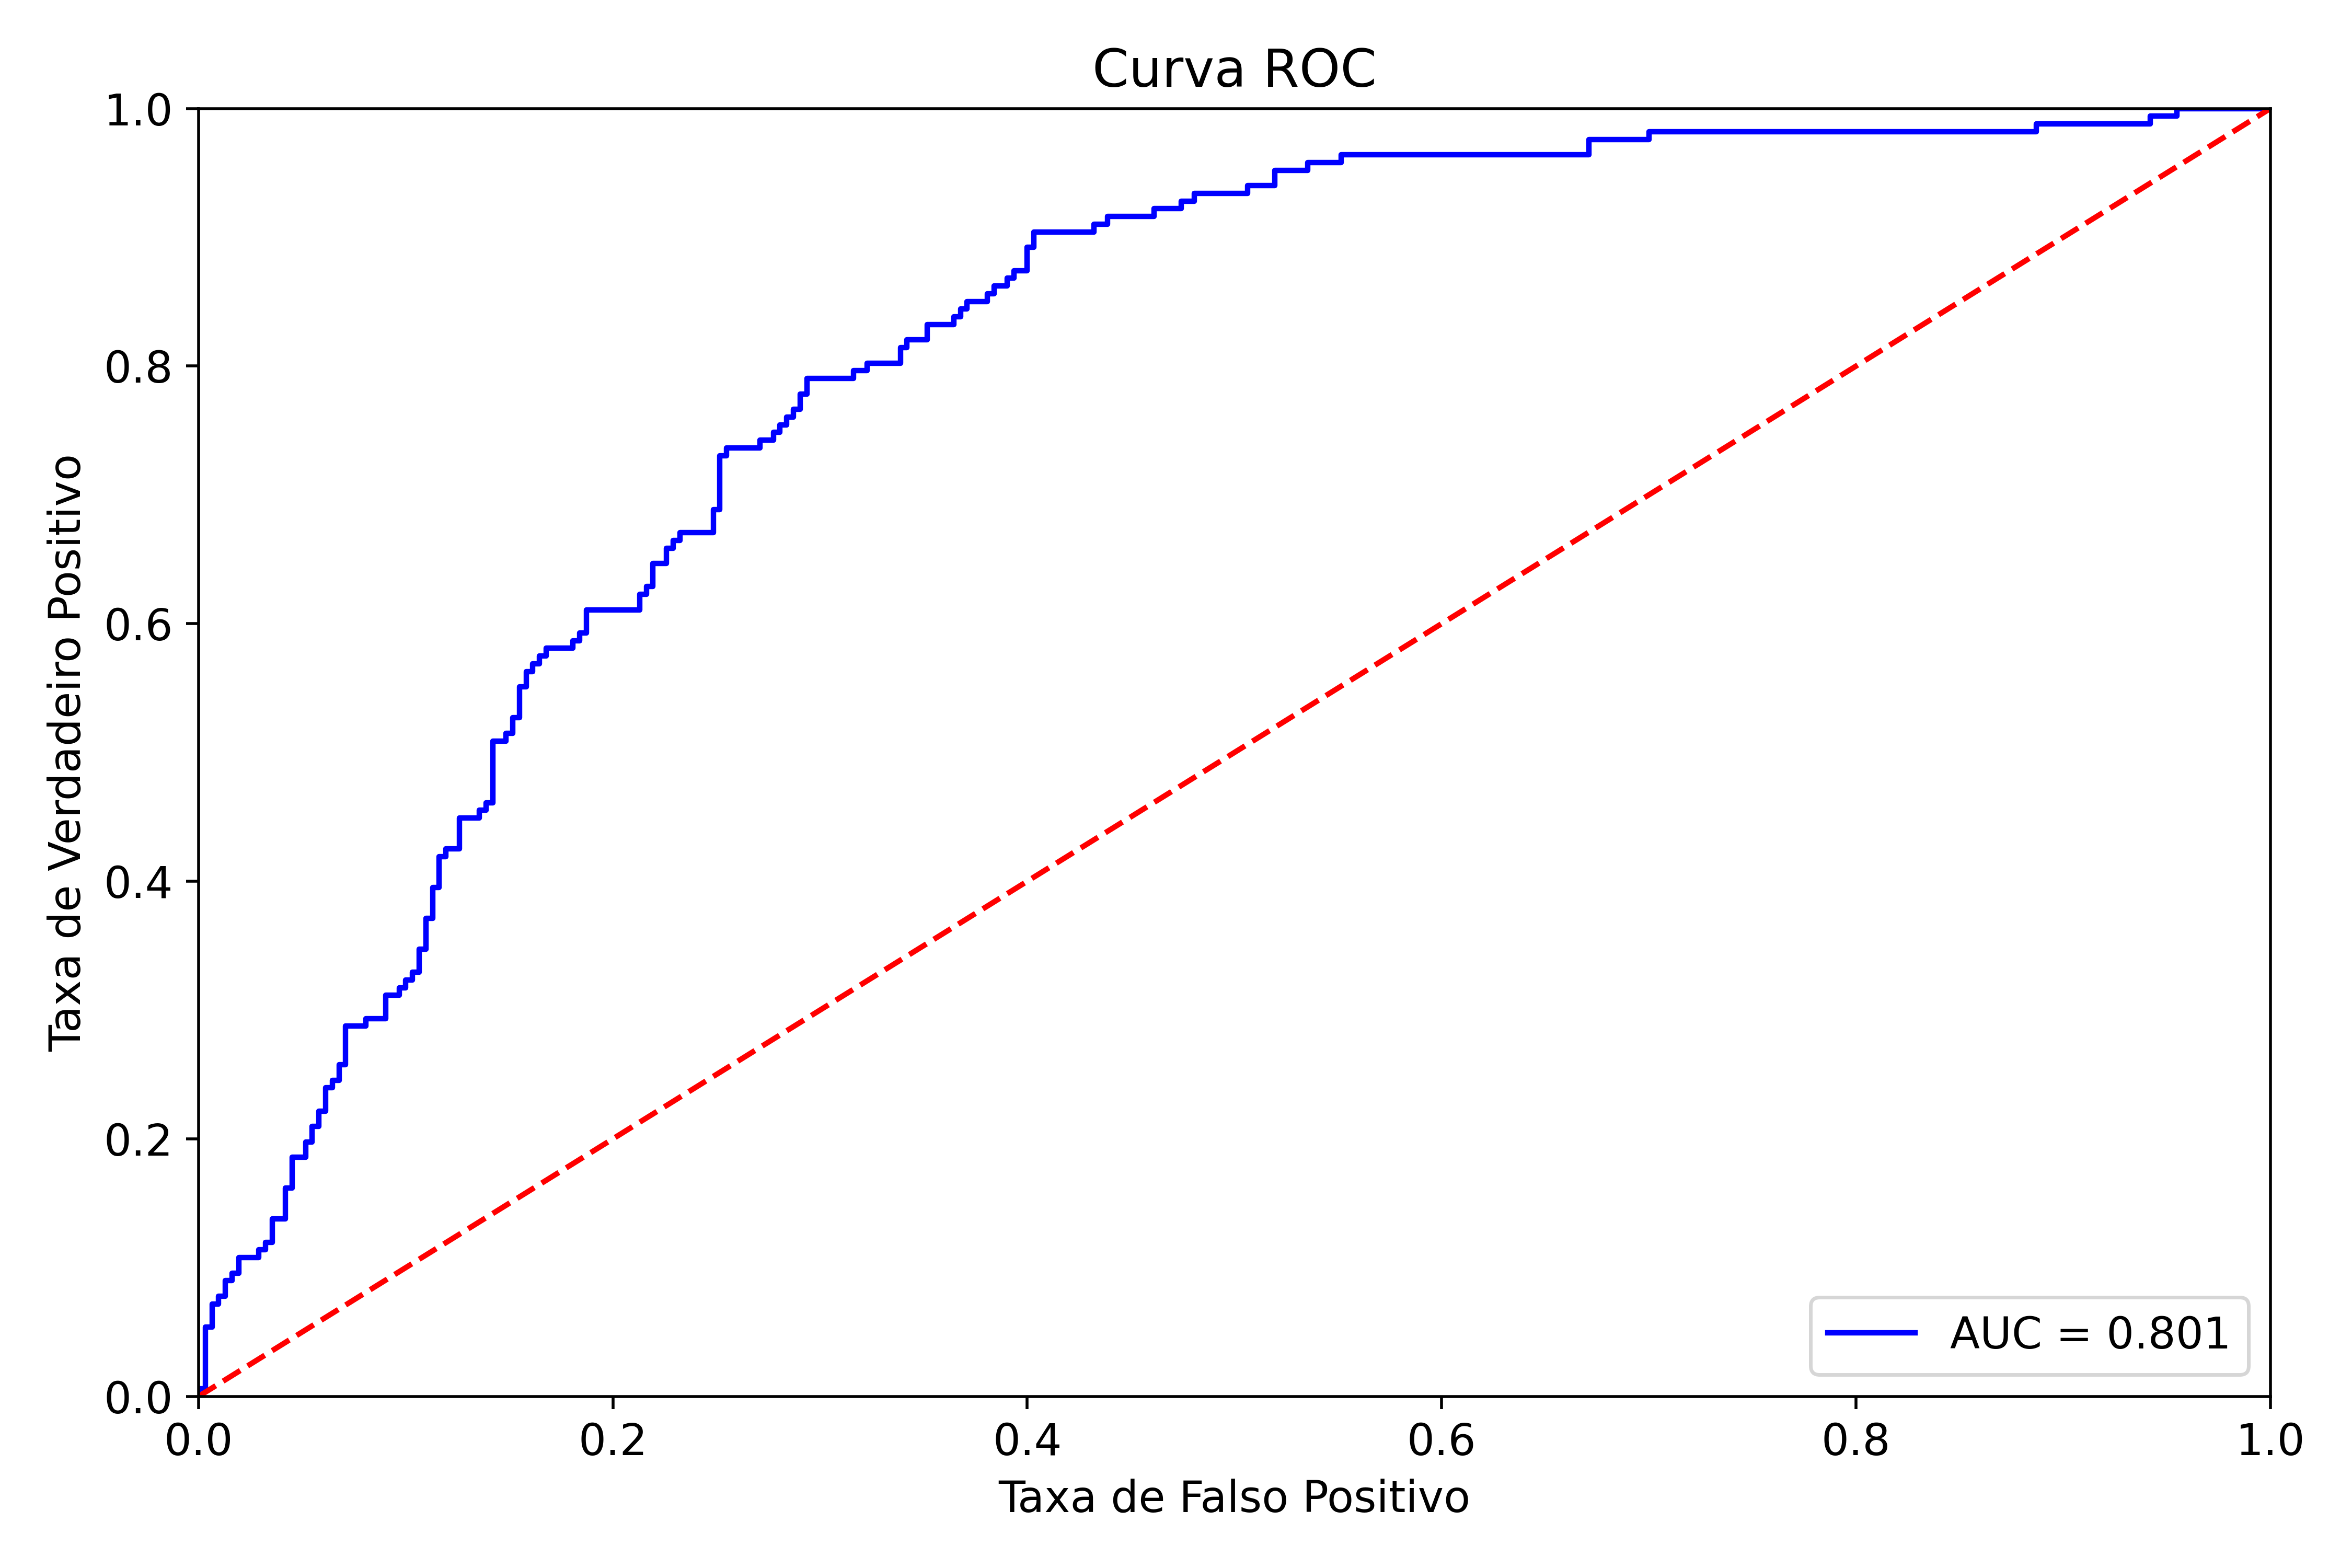
\includegraphics[scale=0.65]{images/nb_roc.png}
    \caption{Curva ROC do modelo de Naïve Bayes aplicado aos dados de teste.}
    \label{fig:nb_roc}
    \end{center}
}
\end{center}
\end{figure}

Vê-se que há uma diferença de performance entre as diferentes bases, que
sobressaí a dispersão observada nas partições do treinamento.
% Este aspecto da supervisão distante será discutido no Capítulo~\ref{chapter:conclusion}.
% TODO: comentar mais pra frente, mas ainda nesse capitulo.
Concluindo a análise do modelo de Naïve Bayes, utilizou-se os dados de treino
para encontrar o limiar de classificação que maximiza o índice SP.
O limiar encontrado teve o valor de $0,88$ e a Figura~\ref{fig:nb_confusion}
apresenta a matriz confusão correspondente a esse valor.
% TODO: comentar alto falso positivo?

\begin{figure}[h!]
\begin{center} {
    \begin{center}
    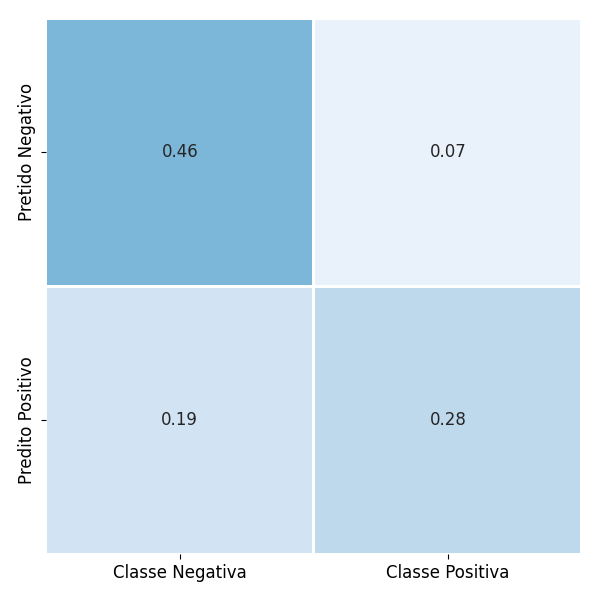
\includegraphics[scale=0.65]{images/nb_cm.png}
    \caption{Matriz confusão do modelo de Naïve Bayes operando no limiar de classificação que maximiza o índice SP.}
    \label{fig:nb_confusion}
    \end{center}
}
\end{center}
\end{figure}

Em seguida, testou-se o classificador por SVM, modelo que obteve melhor
resultados nos testes feitos por \citet{go09}.
O vocabulário utilizado para codificação one-hot foi o mesmo aplicado ao
Naïve Bayes.
Também se aplicou validação cruzada com 10 partições para determinar o melhor
parâmetro de regularização $L_2$.
A Figura~\ref{fig:svm_grid} apresenta os valores de AUC obtidos nos dados de
treino para o intervalo de parâmetro testado.

\begin{figure}[h!]
\begin{center} {
    \begin{center}
    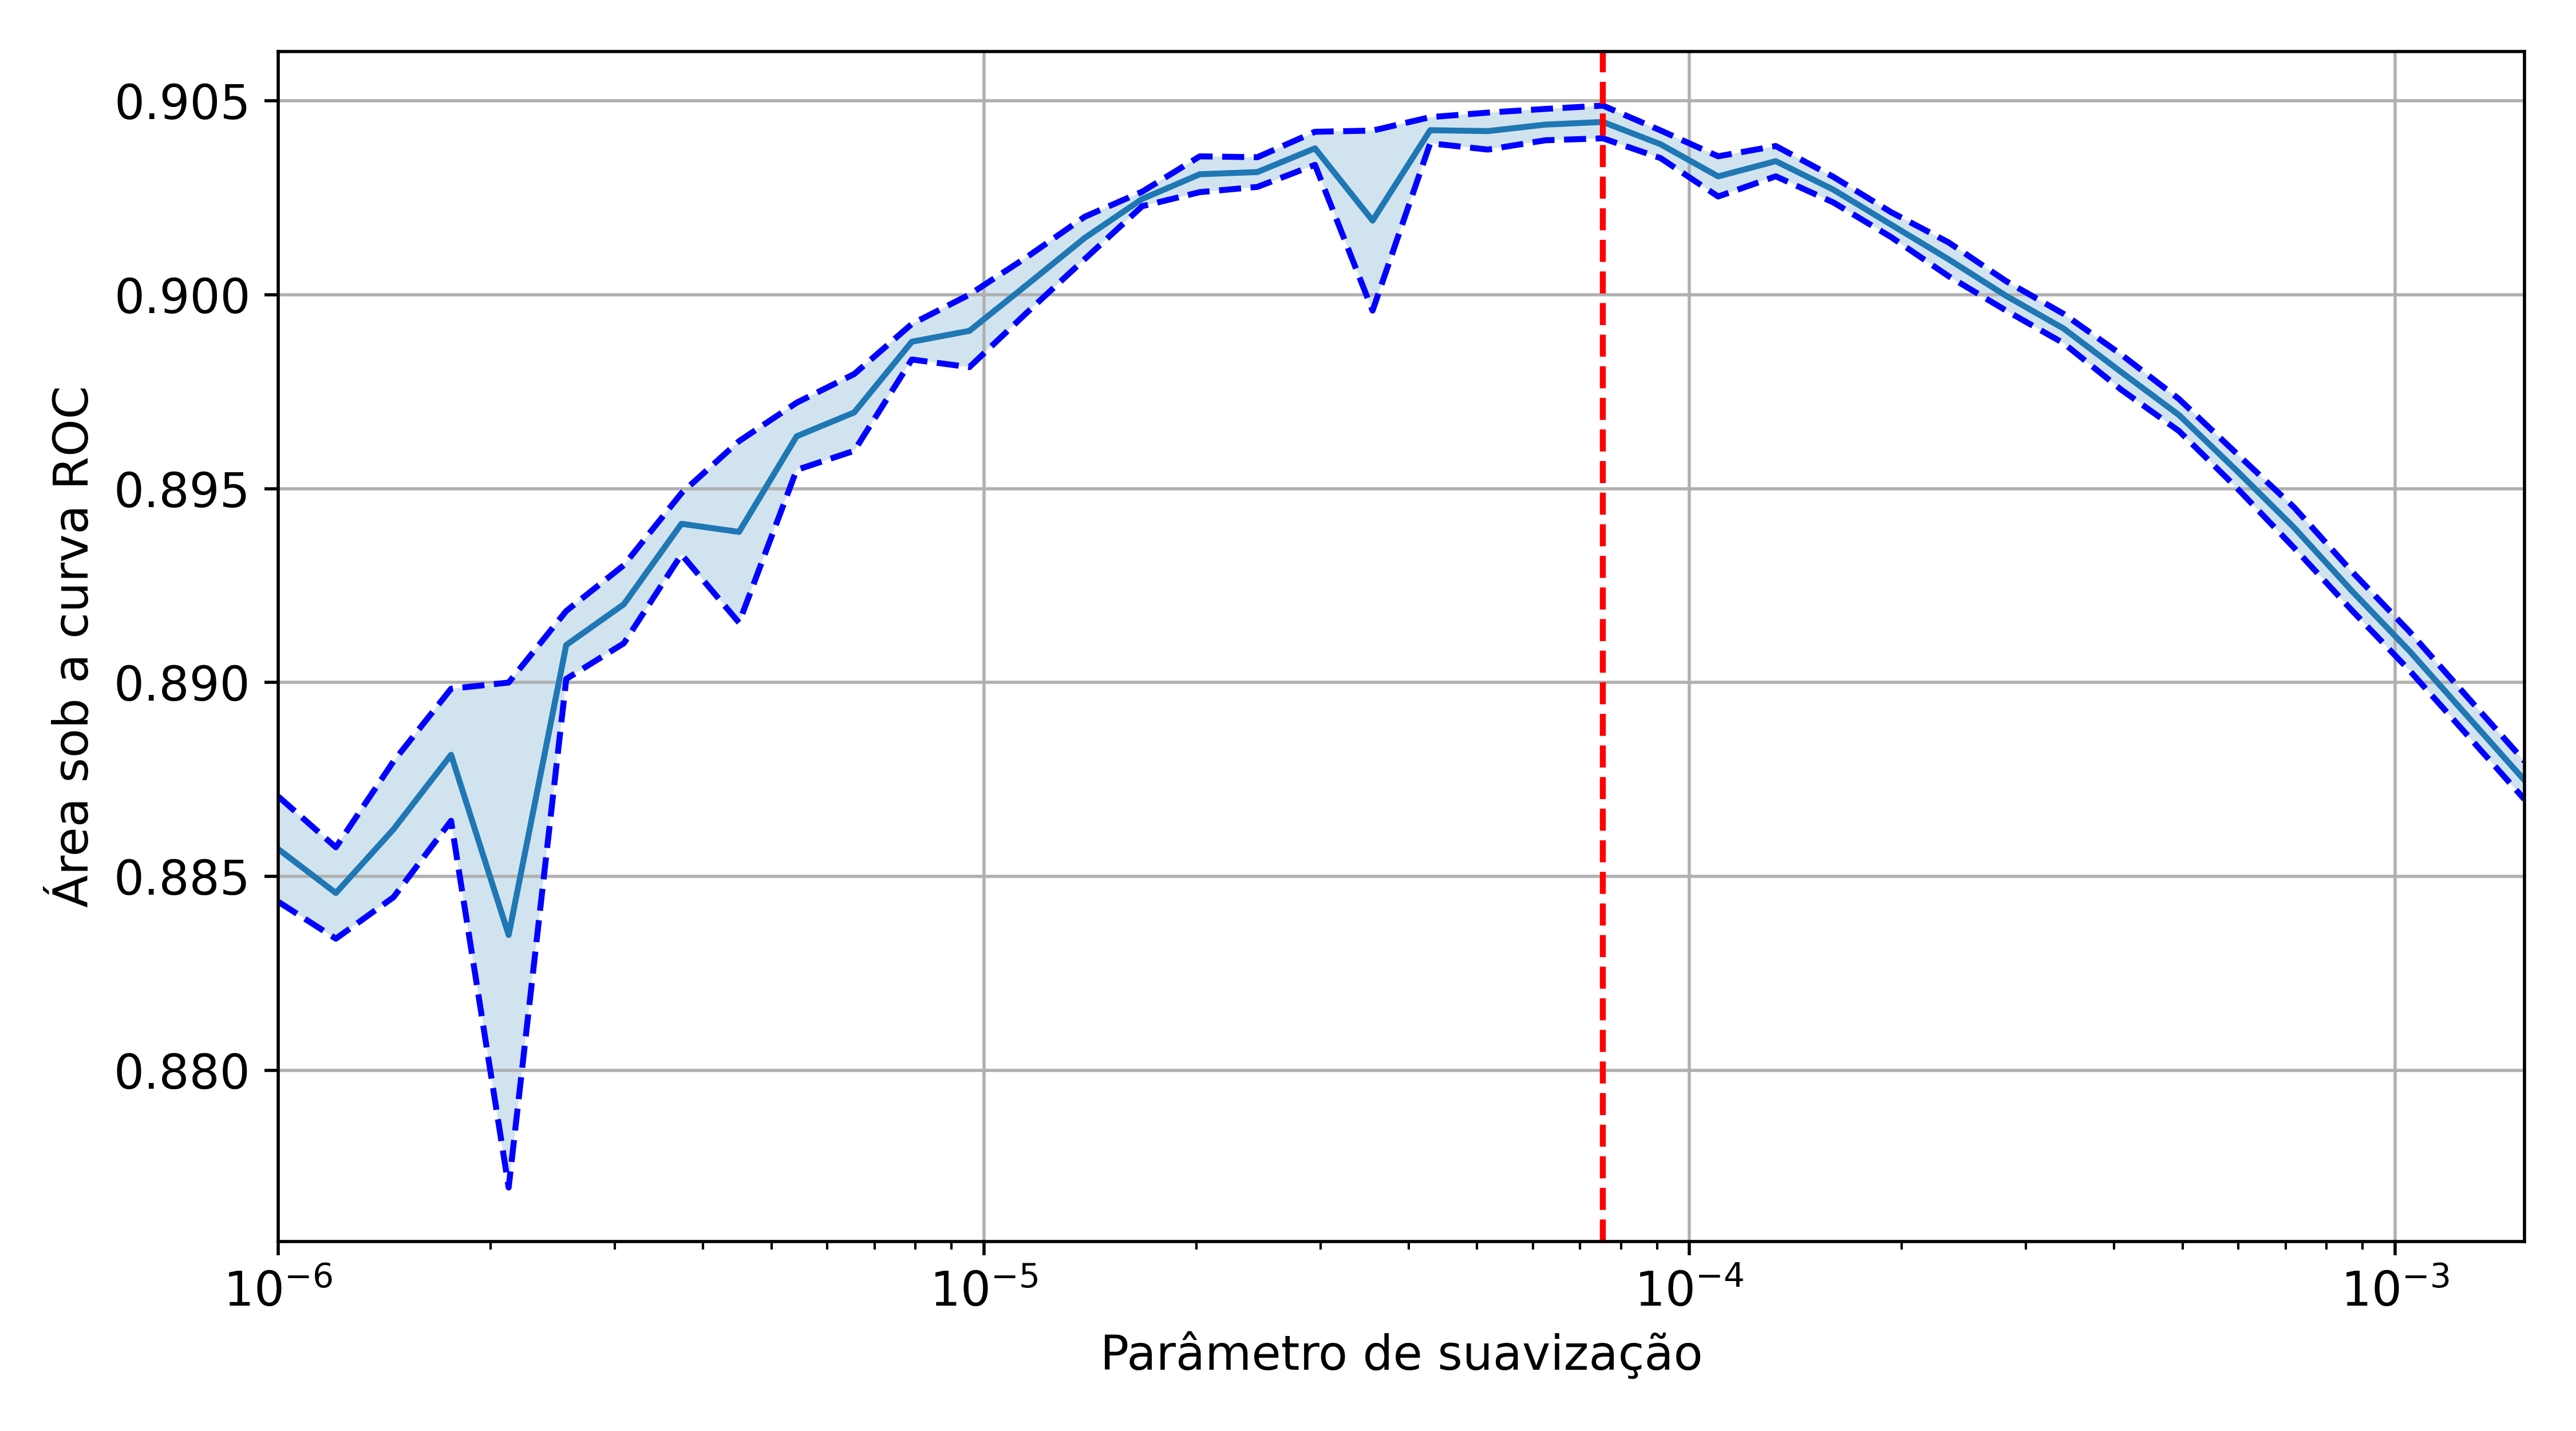
\includegraphics[scale=0.65]{images/svm_grid.png}
    \caption{Resposta do modelo de SVM a variação do parâmetro de regularização.
             A linha cheia representa a média dos valores das 10 partições
             enquanto a área em azul, limitada pela linha hachurada, representa um desvio padrão.
             A linha vertical vermelha ressalta o parâmetro de maior média.}
    \label{fig:svm_grid}
    \end{center}
}
\end{center}
\end{figure}

Observamos que o valor máximo obtido de AUC nos dados de treino foi
$0,904 \pm 0,001$, para o fator de regularização $7\times10^{-5}$.
Porém, ao aplicar o modelo aos dados de teste, a performance do modelo cai
consideravelmente, como vemos na Figura~\ref{fig:svm_roc}, com $0,647$ de área
da curva ROC.

\begin{figure}[h!]
\begin{center} {
    \begin{center}
    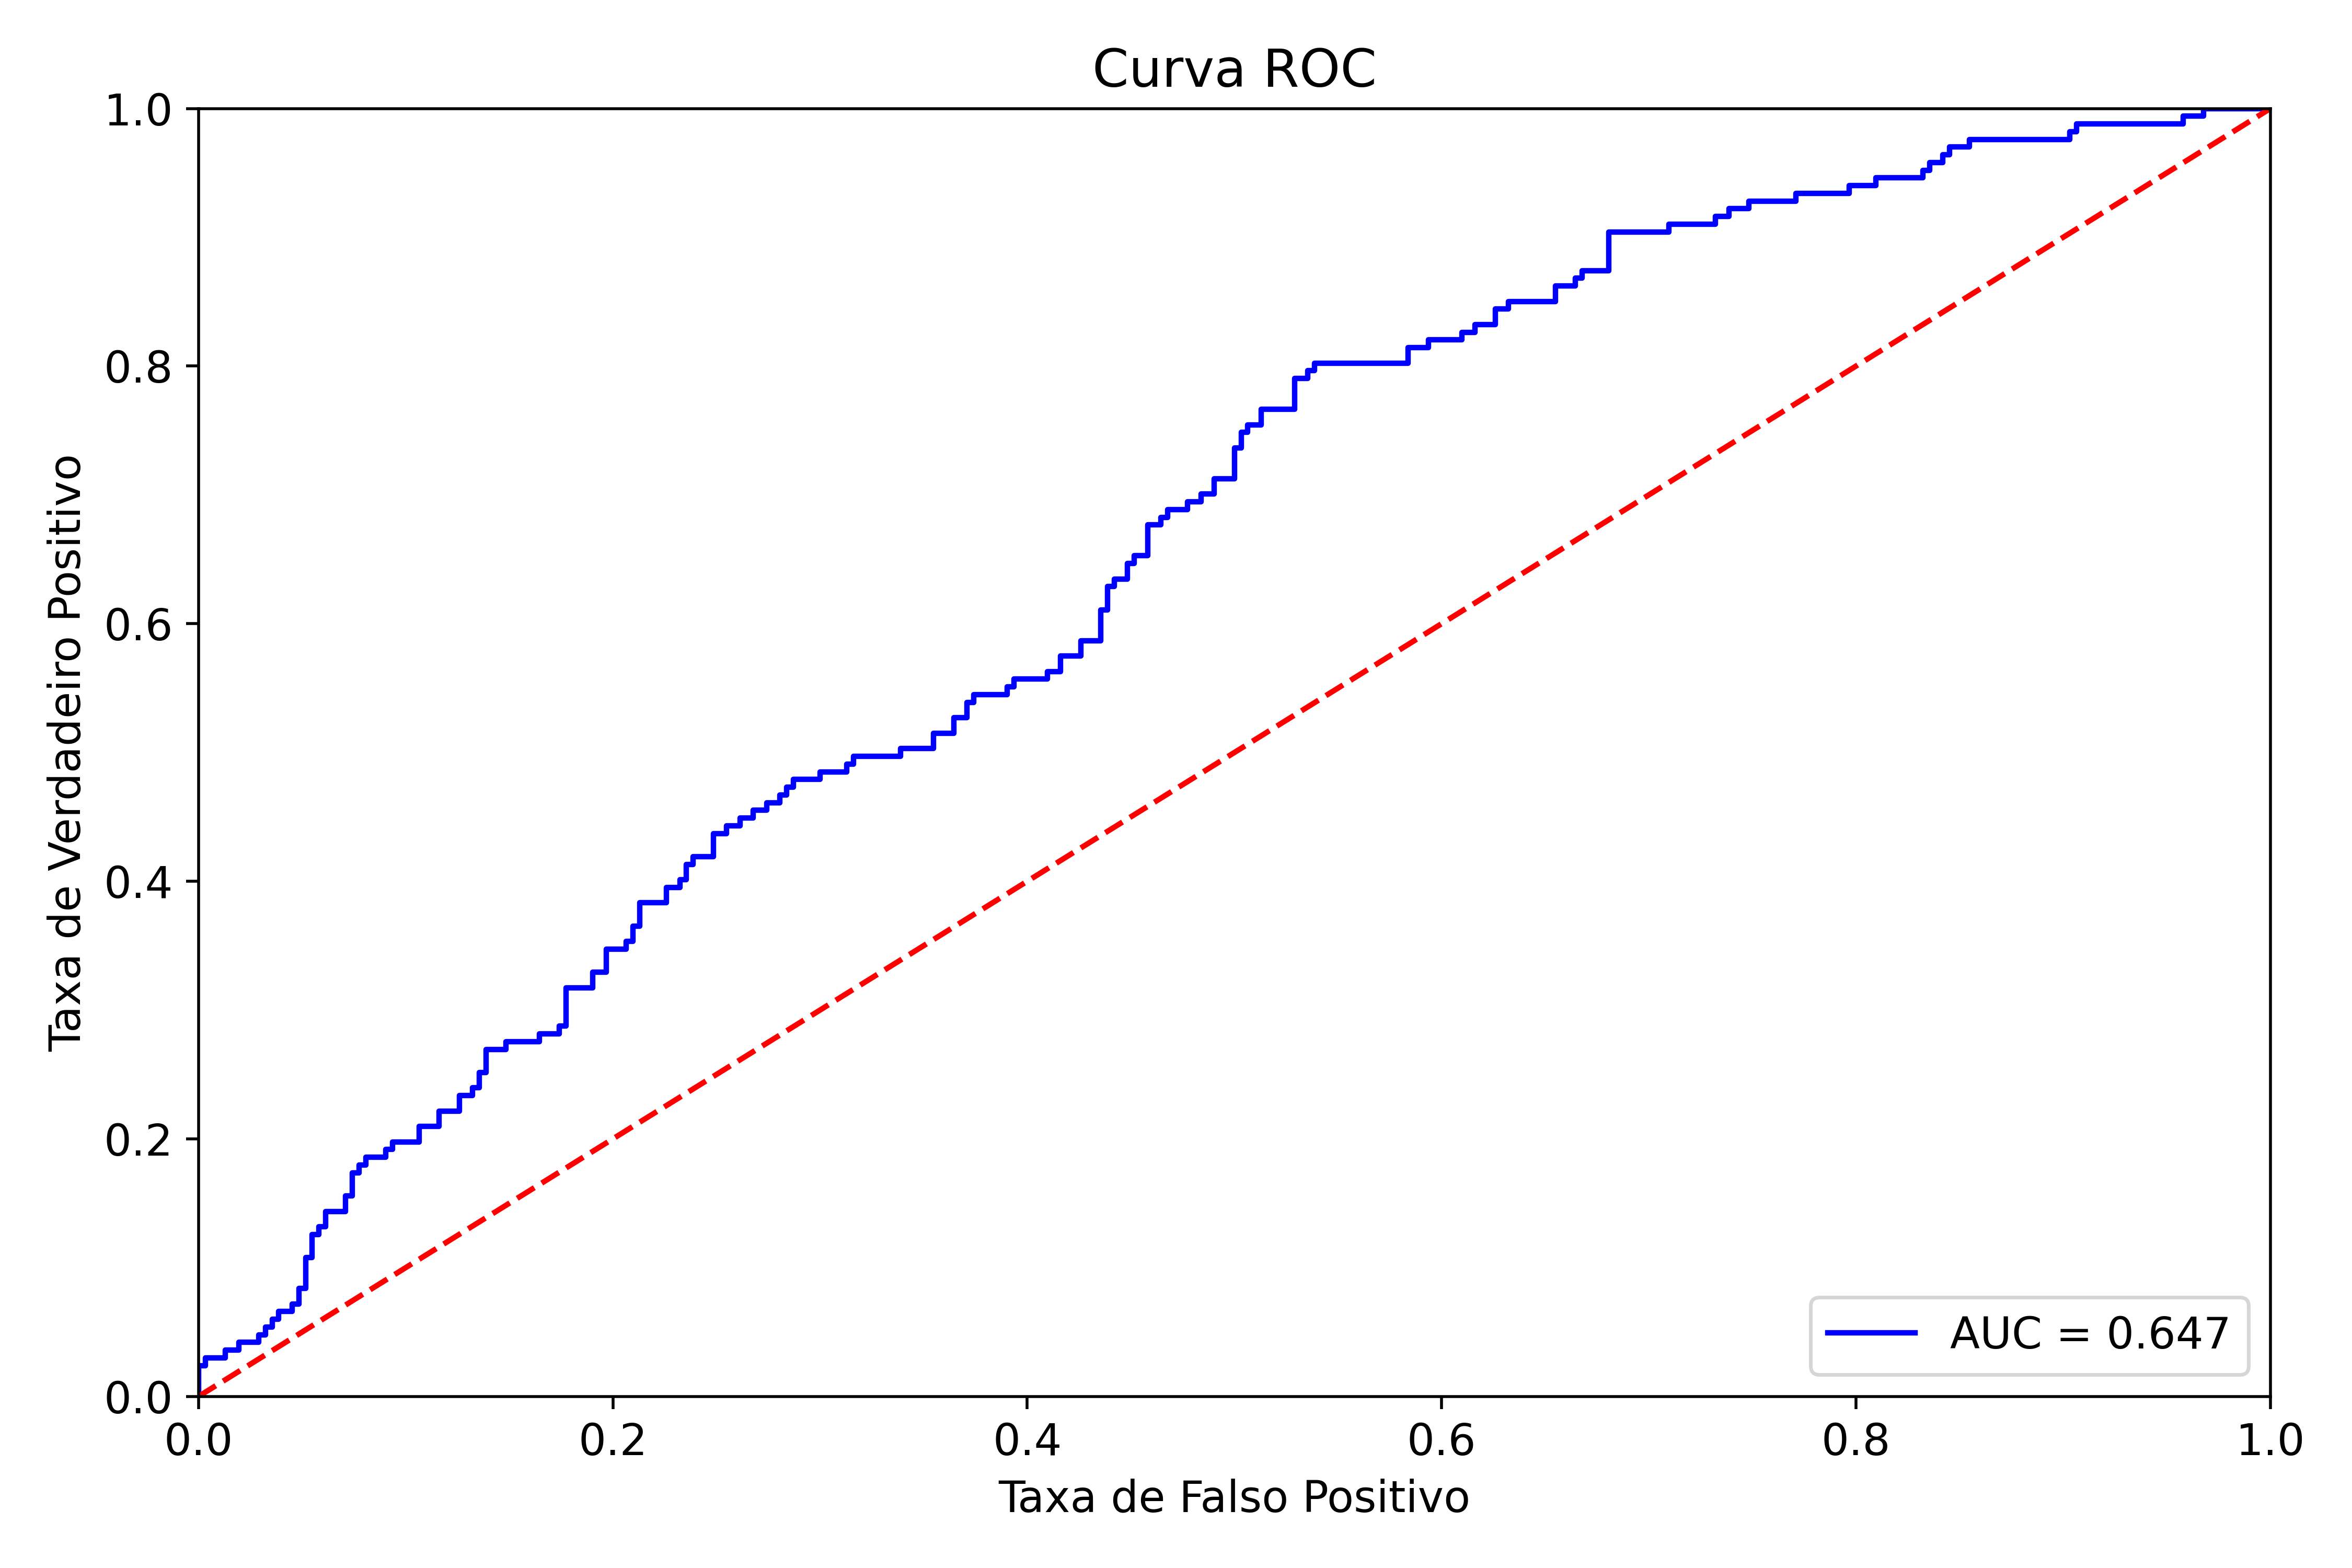
\includegraphics[scale=0.65]{images/svm_roc.png}
    \caption{Curva ROC do modelo de SVM aplicado aos dados de teste.}
    \label{fig:svm_roc}
    \end{center}
}
\end{center}
\end{figure}

O limiar de maior índice SP foi $0,776$, obtendo a matriz confusão
apresentada na Figura~\ref{fig:svm_confusion}.
A matriz confusão mostra que o modelo consegue distinguir elementos da classe
positiva, entretanto, ao ser aplicado em frases negativas o mesmo não conseguiu
performance melhor que escolha aleatória.
Observa-se também que apesar do modelo SVM superar as métricas do modelo de
Naïve Bayes nos dados de treino, SVM generaliza significativamente menos quando
aplicado ao banco de dados de teste.
Apresentando assim uma grande discrepância entre a performance da base anotada
por supervisão distante e a classificada manualmente.

\begin{figure}[h!]
\begin{center} {
    \begin{center}
    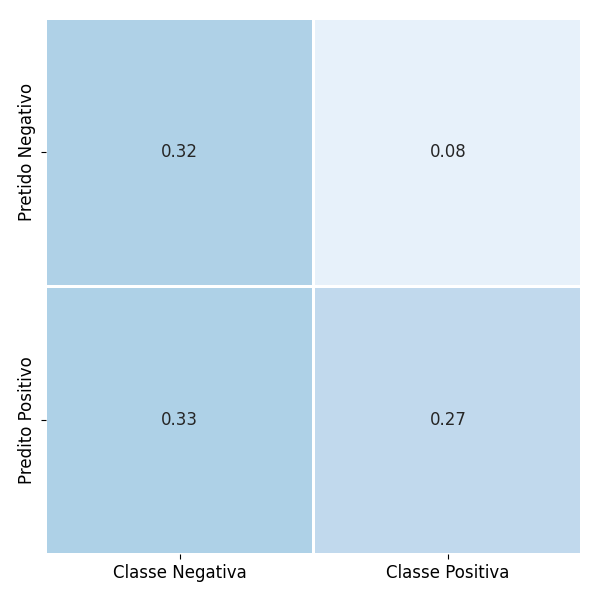
\includegraphics[scale=0.65]{images/svm_cm.png}
    \caption{Matriz confusão do modelo de SVM operando no limiar de classificação que maximiza o índice SP.}
    \label{fig:svm_confusion}
    \end{center}
}
\end{center}
\end{figure}


\section{Classificadores Textuais por Redes Neurais}

Prosseguindo para os classificadores por redes neurais, começamos com o
treinamento da representação de texto.
Realizou-se o treino do \textit{Word2Vec} com os parâmetros
apresentados na Seção~\ref{sec:nlp-classifier}.
O treinamento foi executado até a convergência da função custo.

Obtido o modelo \textit{Word2Vec}, foi realizado o treino dos classificadores de
redes neurais convolucionais.
Algumas das curvas de treinamento são demonstradas na Figura~\ref{fig:cnn_train}.
Observamos que, normalmente, após a terceira época a função custo de treinamento
apresenta uma estabilidade.

\begin{figure}[h!]
\begin{center} {
    \begin{center}
    \includegraphics[scale=0.25]{images/cnn_train.png}
    \caption{Amostras de curvas de treinamento de classificadores por redes neurais
        convolucionais.}
    \label{fig:cnn_train}
    \end{center}
}
\end{center}
\end{figure}

Devido ao \textit{early stopping} cada treinamento acaba em épocas diferentes.
Como aplicamos \textit{dropout} e regularização durante o treinamento temos que
a entropia cruzada de treinamento é mais alta do que a de validação.
Ressaltamos que os treinamentos convergiram para valores parecidos, não
oscilando entre diferentes mínimos locais.

Seguimos com o treinamento do modelo de LSTM, mantendo a entrada com a
representação \textit{Word2Vec}.
A Figura~\ref{fig:lstm_train} apresenta uma amostra dos 10 treinamentos
realizados da rede LSTM.

\begin{figure}[h!]
\begin{center} {
    \begin{center}
    \includegraphics[scale=0.25]{images/lstm_train.png}
    \caption{Amostras de curvas de treinamento de classificadores por redes neurais LSTM.}
    \label{fig:lstm_train}
    \end{center}
}
\end{center}
\end{figure}

Vemos que com LSTM demorou-se mais para atingir convergência, sendo precisas
30 a 50 épocas de treino até a estabilização da função custo.
Observamos também que assim como as redes convolucionais, não houve grande
variação entre os mínimos encontrados pelas diferentes realizações de
treinamento das redes.

Finalmente, utilizaremos o ELMo como forma de representação em conjunto com o
classificador de redes convolucionais.
O alto custo computacional de treinamento desse modelo implicou em algumas
limitações de sua execução.
Obteve-se pesos pré-treinados, portanto, não pode se selecionar a
dimensionalidade da representação.
Neste caso, cada palavra será representada por um vetor de tamanho $1024$.
Também não foi possível fazer múltiplas realizações do treinamento.
A rede convolucional, responsável pela classificação, foi treinada com os mesmos
hiperparâmetros adotados em sua versão com entrada por \textit{Word2Vec}.
A Figura~\ref{fig:elmo_train} apresenta a curva de treinamento do modelo.

% val loss < train loss pq train tem validacao
% https://twitter.com/aureliengeron/status/1110839223878184960

\begin{figure}[h!]
\begin{center} {
    \begin{center}
    \includegraphics[scale=0.45]{images/elmo_cnn_train.png}
    \caption{Curvas de treinamento do modelo com representação ELMo e classificador de CNN.}
    \label{fig:elmo_train}
    \end{center}
}
\end{center}
\end{figure}

\section{Classificadores Multimodais}

Seguimos para a incorporação da informação dos grafos de usuários nos modelos.
Como descrito na Seção~\ref{sec:multimodal-classifier}, o grafo foi reduzido a
sua componente principal para reduzir os requisitos de memória necessários para
o treinamento dos modelos.
O aprendizado foi realizado em duas etapas: aquisição de \textit{embeddings} a
partir de modelagem não-supervisionada do grafo; posteriormente foi realizado o
treinamento em conjunto com os modelos textuais treinados anteriormente.

As redes conjuntas são compostas pelas camadas concatenadas da representação textual
do \textit{tweet} com a representação do grafo do usuário, seguida de 2 camadas
classificatórias de tamanhos respectivamente de $100$ e $32$ neurônios completamente
conectados.
Os pesos das representações do usuário e textuais continuaram a sofrer
\textit{fine-tunning} durante a otimização do modelo.
Assim como nos classificadores textuais, a seleção do limiar de
classificação foi definida pelo ponto de maximização do índice SP.

Começando pelo treinamento da representação por \textit{Locally Linear Embedding}.
Pelo algoritmo depender da matriz de adjacência, que tem custo quadrático em
memória, foi necessário limitar o número de usuários da rede.
Foram selecionados aleatoriamente $10$ mil usuários dentro da subgrafo de
usuários da maior componente conectada para o treinamento do algoritmo.
Foram feitas $10$ realizações do treinamento, cada uma com seu próprio conjunto
de nós selecionados.
O modelo foi treinado para extrair uma representação de dimensão $128$.
Para melhor comparar os diferentes métodos esse número será mantido pelos outros
métodos.
Os usuários que não foram selecionados no sorteio do treinamento tiveram sua
representação no vetor zero.

Posteriormente foram treinados o algoritmo \textit{Node2Vec}.
Mantiveram-se as $10$ realizações do treinamento e o tamanho do vetor de
representação.
Como este algoritmo não depende da matriz de adjacência, foram realizados os
treinamentos considerando todos os usuários presentes na maior componente.
Neste algoritmo consideramos o grafo como não-direcionado.
Os parâmetros de treinamento do algoritmo foram baseados no proposto por
\citet{grover16}.
Os valores de parâmetro $p$ e $q$ de amostragem foram definidos em $1$.
Os passeios aleatórios para definição dos contextos tiveram $80$ passos
de interação e foram feitas $10$ realizações de passeio por vértice.
Os pesos das arestas não foram considerados durante a realização dos passeios
aleatórios.
Utilizou-se janelas de contexto de tamanho $10$ e treinou-se a otimização dos
pesos por $3$ épocas.

Por fim, treinou-se a rede convolucional de grafos (GCN).
Assim como no caso do \textit{Node2Vec} também se utilizou todo o subgrafo
presente na principal componente.
Assim como nos modelos anteriores continuou-se com as $10$ inicializações e o
tamanho da representação dos nós em $128$ dimensões.
Pelo GCN depender de atributos do vértices para o treinamento da representação,
utilizou-se um atributo obtido pelo próprio grafo, o log do grau do nó.
Essa escolha se deu pois não necessita de extrações adicionais de dados.
Outros atributos dos usuários poderiam ter sido incorporados caso houvesse a
disponibilidade desses dados como: número de seguidores, localização,
frequência de uso, etc.
O modelo foi treinado até a finalização por \textit{early stopping}.

% TODO: matrix confusao dos modelos neurais? ou grafico de distribuicao das
% predicoes

Concluímos os experimentos com a Figura~\ref{fig:experiment_results}
consolidando os resultados obtidos por todos experimentos.
Há diversas análises há serem feitas a partir destes resultados.
Primeiramente, observamos que ao contrario do que esperávamos baseados nos
trabalhos referenciados no Capítulo~\ref{chapter:nlp}, entre os modelos
puramente textuais vemos que os baseados em redes neurais obtiveram resultados
piores que as técnicas lineares tradicionais SVM e Naïve Bayes.
Há diferentes hipóteses que podem ser responsáveis por essas diferença.
A representação de palavras avaliadas nos classificadores neurais,
\textit{Word2Vec} e \textit{ELMo}, podem não ter conseguido obter boas
transformações necessárias para a discriminação entre as classes.
Apesar do modelo \textit{Word2Vec} ter se provado eficiente na captação de
contexto sintático e semântico, a grande maioria dos estudos analisados utilizam
textos em formatos longos como artigos jornalistico.
Há também a possibilidade de que a base de \textit{tweets} disponível para o seu
treinamento não tenha sido suficiente para o modelo adquirir estatística
suficiente dos dados.
A representação pelo modelo \textit{ELMo}, por sua vez, foi treinada com artigos
da Wikipedia.
A diferença de linguagem entre esse meio e as redes sociais pode ser um dos
fatores responsáveis pela não reprodução dos bons resultados da técnica nesta
base de dados.
A vantagem das técnicas de classificação menos complexas pode demonstrar ainda
uma dificuldade no treinamento de dados provindos de textos curtos e informais
ou a necessidade de volumes maiores de dados de treinamento do que os coletados
para esse experimento.

\begin{figure}[h]
\begin{center} {
    \begin{center}
    \includegraphics[scale=0.35]{images/experiment_results.png}
    \caption{Comparativo entre modelos textuais e multimodais apresentados nesse
             trabalho. A figura apresenta a área sob a curva ROC dos modelos
             avaliados quando aplicados aos dados de teste. Os 5 modelos a esquerda
             são os resultados dos classificadores puramente textuais enquanto os 6
             modelos a direita são as combinações avaliadas dentre os modelos multimodais.}
    \label{fig:experiment_results}
    \end{center}
}
\end{center}
\end{figure}

Adicionalmente, observa-se que acrescer as representações dos vértices de
usuários resultou em performance variadas para os diferentes modelos, não
havendo conclusão clara sobre sua eficiência.
Comparando os resultados a partir do modelo de CNN, vemos que os experimentos
que incluíram os dados do grafo tiveram média de AUC acima do valor médio
do classificador puramente textuais.
Os modelos compostos demonstraram uma menor variação de resultados, com desvio
padrão significativamente menor do que o modelo puramente textual.
Dentre as diferentes técnicas de representação do grafo houve pouca diferença
entra a escolha.
A representação por GCN apresentou maior média, entretanto, sua média ainda fica
dentro da faixa de um desvio padrão comparado aos modelos com representações por
LLE e \textit{Node2Vec}.

Analisando os classificadores multimodais com base na rede LSTM observamos
comportamento distinto do obtido com a rede convolucional.
Neste caso, o modelo textual superou os modelos compostos.
As representações de grafo por LLE e GCN obtiveram resultados semelhantes.
Porém, a combinação de LSTM com \textit{Node2Vec} superou significativamente
todas outras combinações de modelos multimodais.
Ainda assim, a rede LSTM pura obteve média levemente maior apesar de estar na
faixa de um desvio padrão de diferença do modelo composto com o
\textit{Node2Vec}.

O fato dos modelos multimodais não terem superado significativamente os modelos
textuais pode ter diferentes interpretações.
A escolha de caracterizar os usuários a partir de suas representações do grafo
de retweets pode ser restritiva demais para capturar informações relevantes dos
mesmos.
Complementarmente, é possível que o usuário não contenha informação discriminante
o suficiente para a tarefa de análise de sentimento a ponto de ter maiores
benefícios no resultado.

Por fim, observamos que a supervisão distante a partir de \textit{emoticons} foi
capaz de extrair informação para o treinamento de classificadores visto que
conseguimos modelos com AUC acima da faixa de escolha aleatória.
Entretanto, as matrizes confusão apresentadas nesse capítulo demonstram uma
grande diferença de eficiência entre as classes.
Os modelos tiveram maiores dificuldades em discernir \textit{tweets} da classe
positiva.
Este fenômeno pode ser entendido como resultado da seleção de \textit{emoticons}
positivos serem pouco representativos.
Também pode-se considerar a possibilidade de textos sarcásticos contendo
\textit{emoticons} positivos terem impactado na discriminação dessas mensagens.

% diferente do esperado nlp
% diferente do esperado mixed
% faltou base de treino?
% nao funciona bem em texto curto e informal
% supervised sendo ruim pra modelos complexos?
% problema so nos positivos, pode ser a selecao de emoticon
% problema na representacao de palavras? w2v e elmo
% retweet nao representando bem o usuario?
% TODO: comentar alta taxa de falso positivo do modelo e como isso pode ser consequencia do treinamento semi supervisionado

% FIZ UM BACKUP DE MODELS E JOGUEI EM /mnt/models
